\documentclass{article}

\usepackage{graphicx}
\usepackage{tikz}
\usepackage{tikzsymbols}
\usetikzlibrary{calc,patterns,shapes.geometric}
\pagestyle{empty}
\usepackage[margin=0pt]{geometry}
\geometry{papersize={14in,12in}}

\def\centerarc[#1](#2)(#3:#4:#5){\draw[#1] ($(#2)+({#5*cos(#3)},{#5*sin(#3)})$) arc (#3:#4:#5);}

\begin{document}
	\begin{figure}
		\centering
		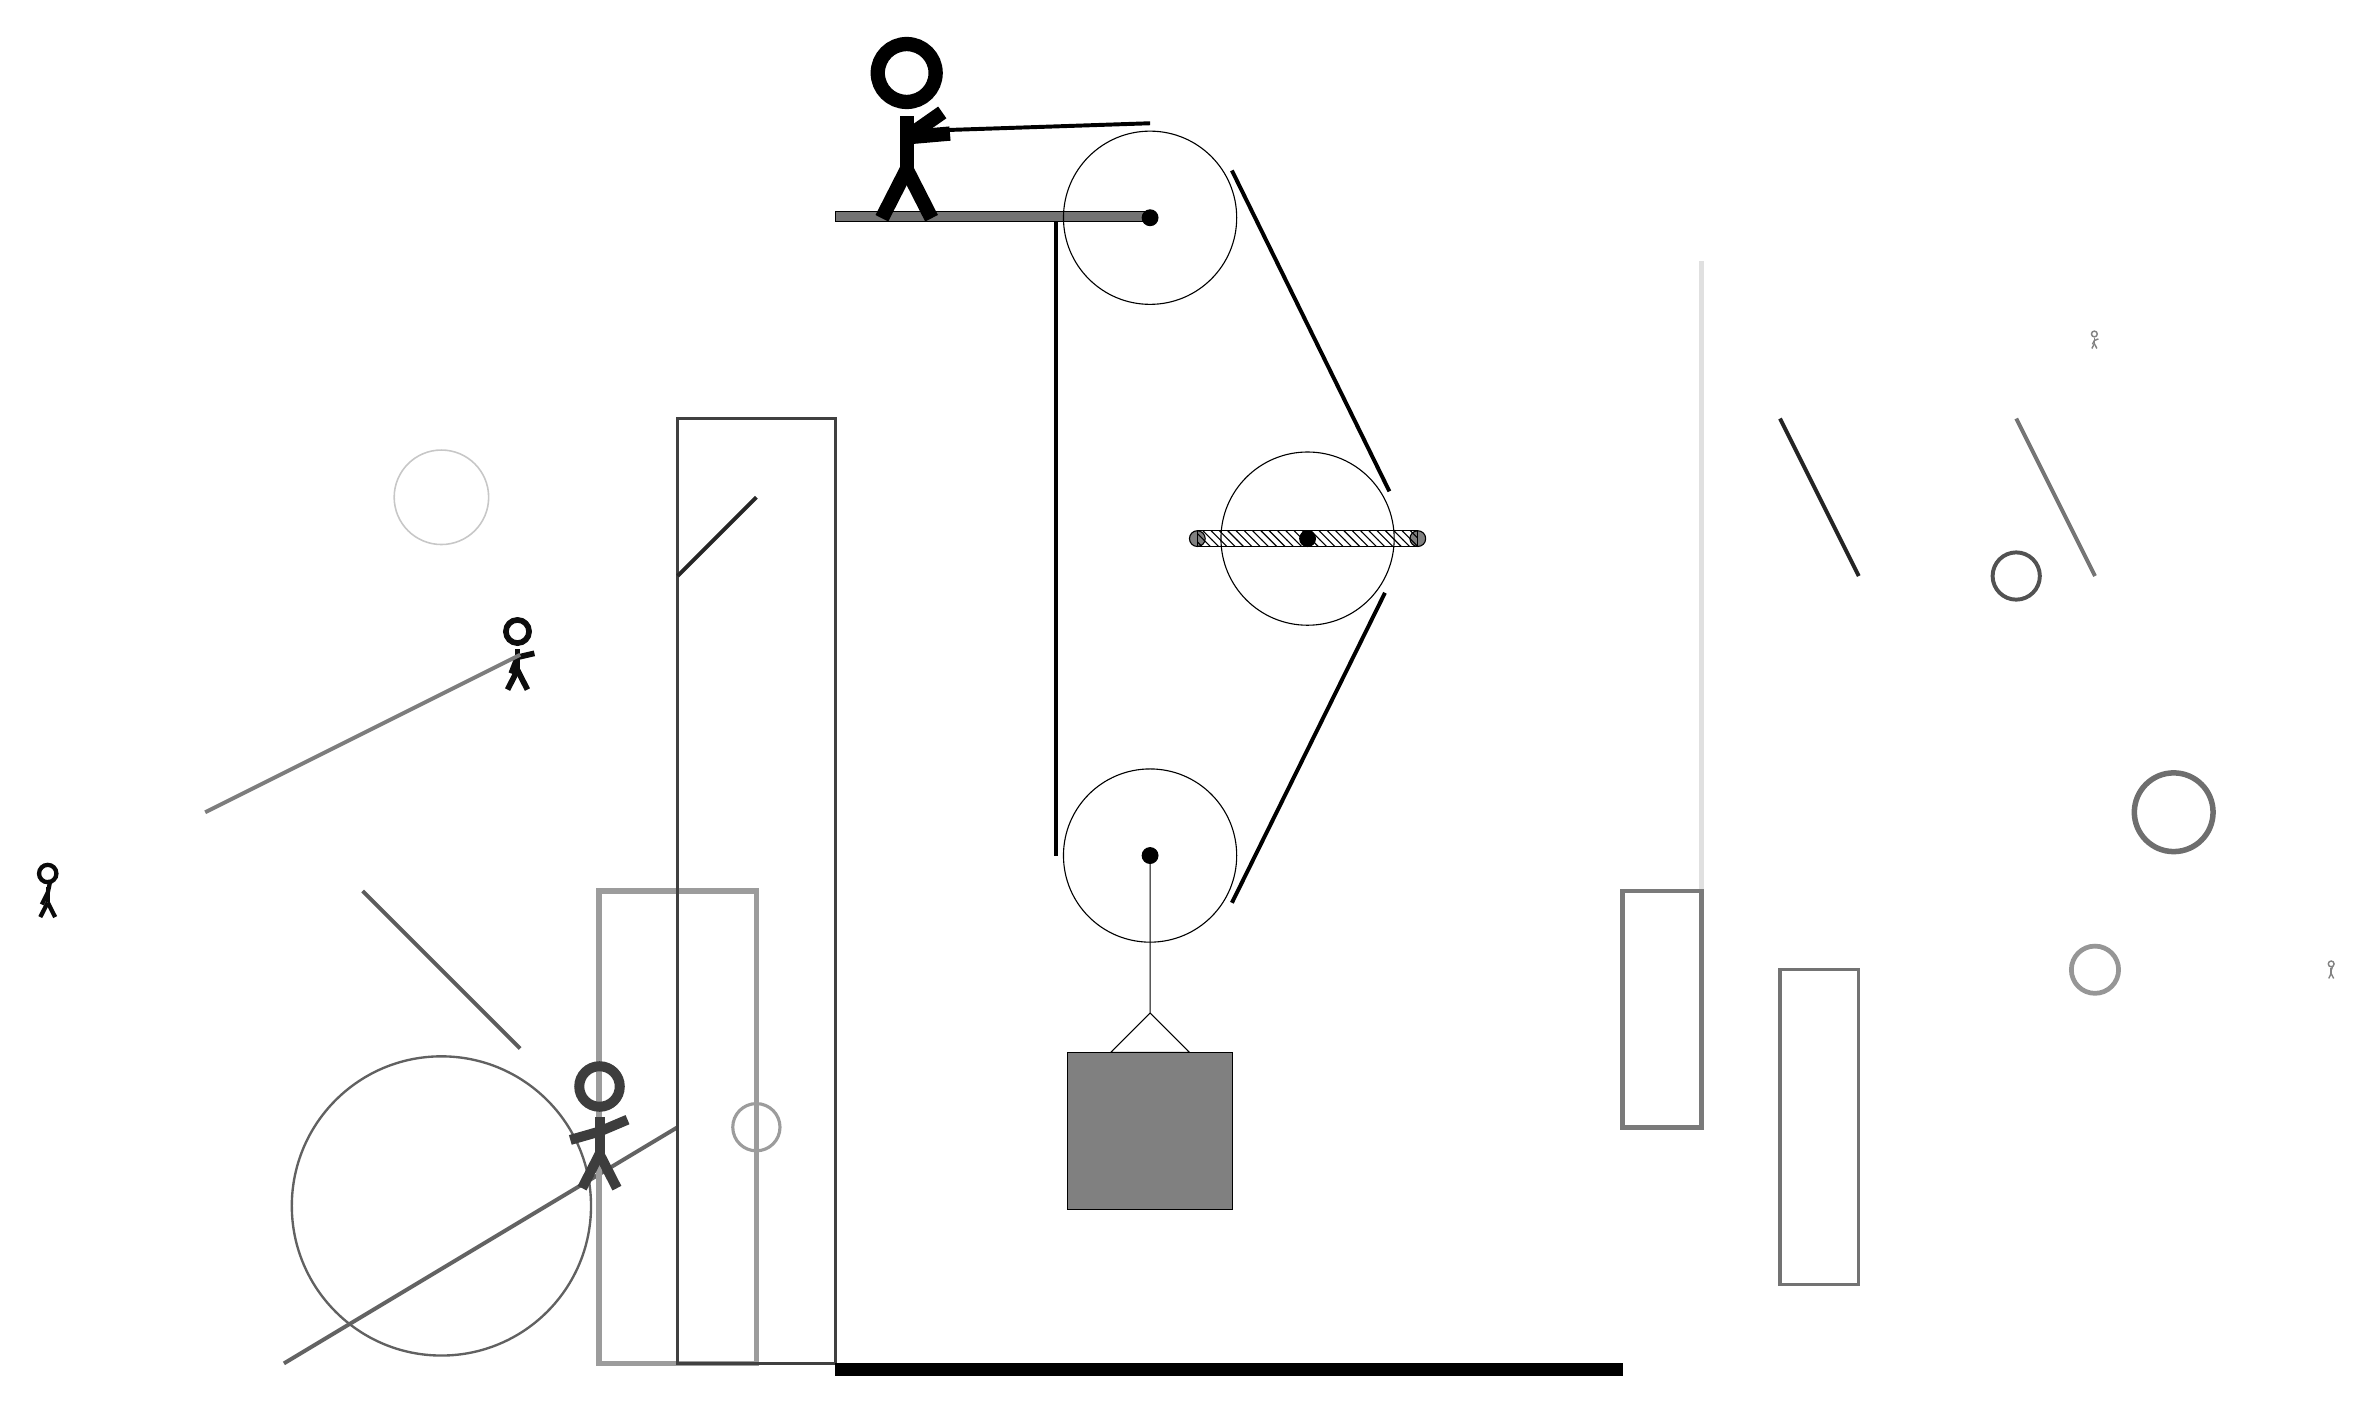
\begin{tikzpicture}
			%%%%% START %%%%%
			
			\draw[fill=black!55] (-2, 11.5) rectangle (2, 11.625);
			
			\draw (2, 3.45) circle (1.1);
			\draw[fill=black] (2, 3.45) circle (0.1);
			
			\draw (2, 11.55) circle (1.1);
			\draw[fill=black] (2, 11.55) circle (0.1);
			
			\draw[fill=white](4, 7.475) circle (1.1);
			\draw[fill=black] (4, 7.475) circle (0.1);
			\draw[fill=black!50] (2.6, 7.475) circle (0.1);
			\draw[fill=black!50] (5.4, 7.475) circle (0.1);
			\draw[pattern=north west lines, pattern color=black] (2.6, 7.575) rectangle (5.4, 7.375);
			
			\draw (2, 3.45) -- (2, 1.45) -- (1.5, 0.95) -- (2.5, 0.95) -- (2, 1.45);
			\draw[fill=black!50] (0.95, 0.95) rectangle (3.05, -1.05);
			
			\draw [line width=0.2mm, color=black!22](-7, 8) circle (0.6);
			
			\draw [line width=0.7mm, color=black!57](15, 4) circle (0.5);
			\draw [line width=0.3mm, color=black!59](12, 6) circle (0.0);
			\draw[line width=0.6mm, color=black!12] (9, 0) rectangle (9, 11);
			\draw[line width=0.5mm, color=black!64](-6, 1) -- (-8, 3);
			\draw[line width=0.5mm, color=black!61](-4, 0) -- (-9, -3);
			
			\draw[line width=0.5mm, color=black!54](13, 9) -- (14, 7);
			\draw [line width=0.3mm, color=black!62](-7, -1) circle (1.9);
			\draw[line width=0.2mm, color=black!41] (-2, -2) rectangle (-2, 7);
			\draw [line width=0.5mm, color=black!68](13, 7) circle (0.3);
			\node[line width=0.5mm, color=black!49] at (14, 10) {\Strichmaxerl[1][63][20]};
			
			\draw[line width=0.4mm, color=black!55] (10, 2) rectangle (11, -2);
			\draw[line width=0.7mm, color=black!39] (-3, 3) rectangle (-5, -3);
			
			\node[line width=0.7mm, color=black!95] at (-6, 6) {\Strichmaxerl[4][69][13]};
			\node[line width=0.2mm, color=black!49] at (17, 2) {\Strichmaxerl[1][82][70]};
			\draw [line width=0.6mm, color=black!41](14, 2) circle (0.3);
			\draw[line width=0.4mm, color=black!75] (-2, -3) rectangle (-4, 9);
			\node[line width=0.7mm, color=black!76] at (-5, 0) {\Strichmaxerl[7][16][23]};
			\draw[line width=0.5mm, color=black!86](11, 7) -- (10, 9);
			\draw[line width=0.5mm, color=black!51](-6, 6) -- (-10, 4);
			\draw [line width=0.4mm, color=black!39](-3, 0) circle (0.3);
			
			\draw[line width=0.6mm, color=black!52] (8, 0) rectangle (9, 3);
			\node[line width=0.2mm, color=black!96] at (-12, 3) {\Strichmaxerl[3][63][78]};
			\draw[line width=0.5mm, color=black!85](-3, 8) -- (-4, 7);
			
			\draw[line width=0.5mm] (0.8, 11.5) -- (0.8, 3.45);
			\centerarc[line width=0.5mm](2, 3.45)(180:330:1.2000000000000002);
			\draw[line width=0.5mm](3.0392, 2.85) -- (4.983, 6.7867);
			\centerarc[line width=0.5mm](4, 7.475)(390:325:1.2000000000000002);
			\draw[line width=0.5mm](5.0392, 8.075) -- (3.0392, 12.15);
			\centerarc[line width=0.5mm](2, 11.55)(30:90:1.2000000000000002);
			\draw[line width=0.5mm](2, 12.75) -- (-1, 12.65);
			
			\node at (-1, 12.65) {\Strichmaxerl[10][-175][35]};
			
			\draw[fill=black] (-2, -3) rectangle (8, -3.15);
			
			%%%%% END %%%%%
		\end{tikzpicture}
	\end{figure}	
\end{document}